\chapter{Research}
Before I start to design my traffic light control system, I need to research existing designs, to understand both how they work and how they are controlled.

\section{How Traffic Lights Work}
Traffic lights are generally divided into two categories, they will either be based off of a timing circuit or they will have some form of vehicle sensor which will trigger the changing of the lights. Each of these have their own pros and cons. Sometimes a combination of the two is preferred.

\subsection{Systems with Vehicle Sensors}
Traffic light control systems which are based off of a vehicle sensor or sensors alone are generally inadequate for for junctions in areas with a higher population density. Using the diagram below (fig. \ref{fig:bridgeDiagram} as an example; the blue cars are able to cross the bridge, but as there are blue cars constantly arriving at traffic light set A, the system doesn't see that there are cars waiting at traffic light set B therefore it doesn't change. This means that there is a pile up of cars at traffic lights B.
\begin{figure}[H]
    \centering
    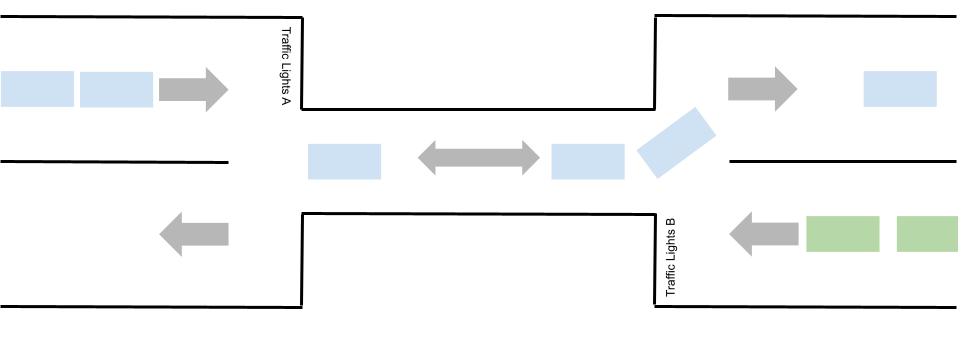
\includegraphics[width=0.8\textwidth]{images/Bridge diagram.png}
    \caption{Diagram of traffic flow over a bridge}
    \label{fig:bridgeDiagram}
\end{figure}

\subsection{Systems with Timers}
Traffic light control systems which are based off of a timer alone are generally more suited for areas which receive higher levels of traffic. This is because they allow one set of traffic to move for a set length of time then allow the other set to move for a set length of time, then repeats.

\subsection{Systems with Timers and Vehicle Sensors}
Traffic light control systems which are based off of a timer and vehicle sensor(s) are the most efficient, however with the added efficiency comes additional complexity. This is the best type of system as (using the diagram in Fig. \ref{fig:bridgeDiagram}) the system would be able to tell that the blue cars have had a chance to go and there are green cars waiting therefore it can let the green cars go.


\section{Traffic Light Controlled Junctions}
There are a number of different types of traffic light and pedestrian crossing systems\footnote{https://www.highwaycodeuk.co.uk/rules-for-pedestrians-crossings.html}, each has a different priority pattern and each uses a different combination of vehicle/pedestrian sensors and timing systems.

\subsection{EXAMPLE 1: Two-Way Traffic Lights}
\begin{figure}[H]
    \centering
    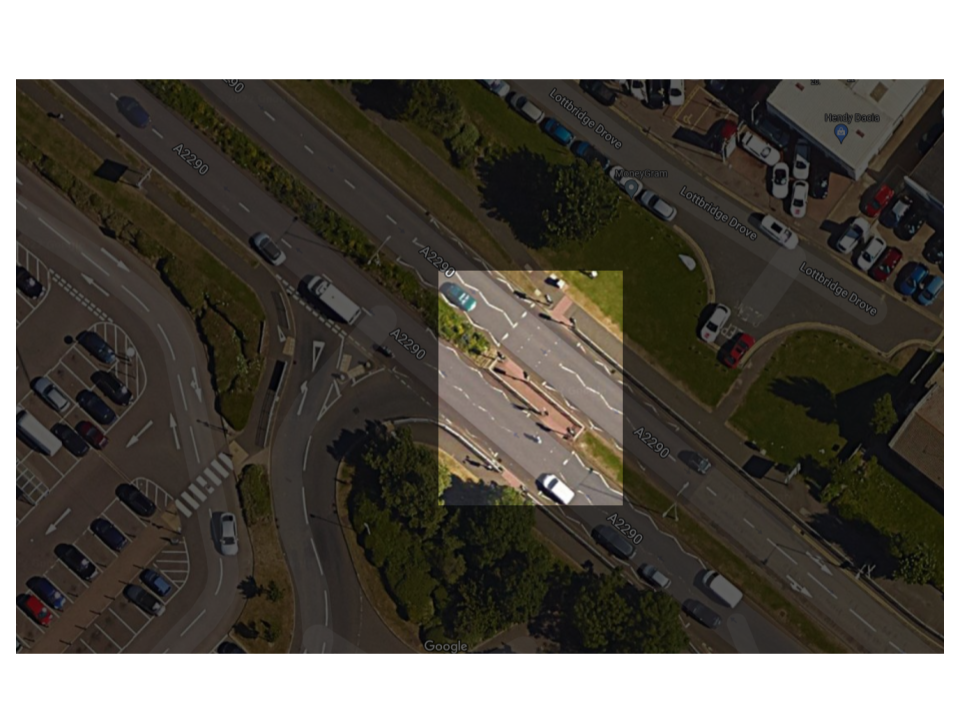
\includegraphics[width=0.8\textwidth]{images/Simple TL junction outside tesco.png}
    \caption{Image of the two-way junction}
    \label{fig:tesoTrafficLights}
\end{figure}
\noindent \textit{Data from Google Maps (2022). Available from:\\ https://www.google.com/maps/@50.7865833,0.3056209,74m/data=!3m1!1e3 [Accessed 13 03 2022]}\newline

\noindent This junction has two identical sections to it. Each has a set of traffic lights to stop a single carriageway of traffic and a pedestrian crossing to allow pedestrians to cross the dual carriage which this is situated on. Due to the fact that this is on a dual carriageway, it can safely be assumed that this traffic light system is controlled by the pedestrian crossing alone, without any vehicle sensors or timing control systems. This assumption would work by the pedestrian pressing the button which indicates to the system that they are ready to cross then the system waiting a set length of time, allow the pedestrians to cross for a set length of time then return to a green light for the traffic.

\subsection{EXAMPLE 2: Complex Junction}
\begin{figure}[H]
    \centering
    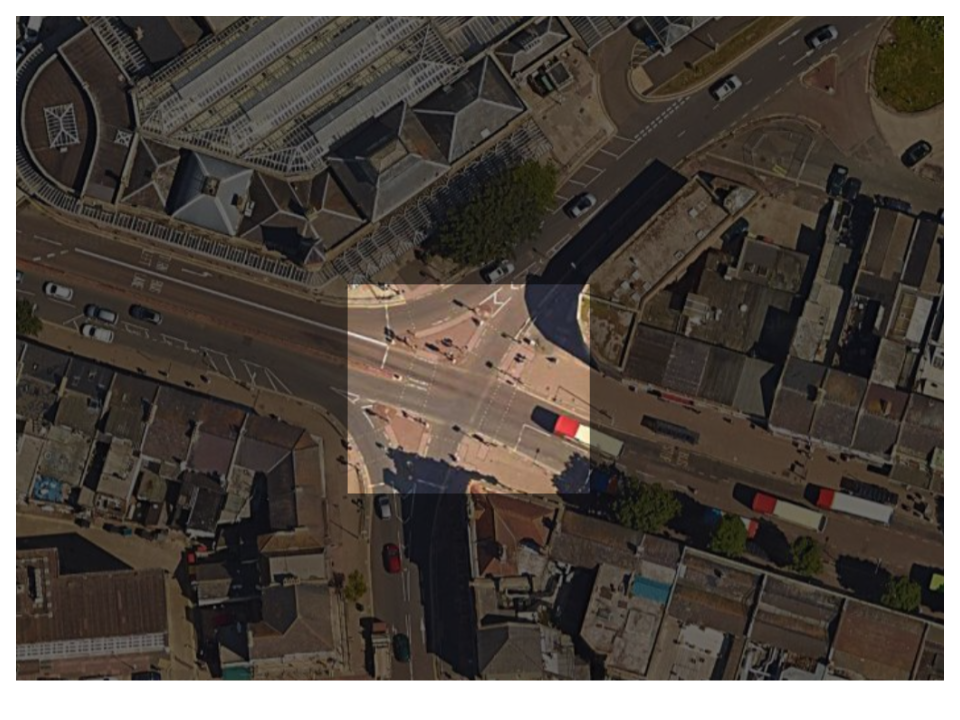
\includegraphics[width=0.8\textwidth]{images/Complex junction.png}
    \caption{Image of the complex junction}
    \label{fig:complexJunction}
\end{figure}
\noindent \textit{Data from Google Maps (2022). Available from:\\ https://www.google.com/maps/@50.7690679,0.2817194,121m/data=!3m1!1e3 [Accessed 13 03 2022]}\newline

\noindent This is a much more complicated junction where there are multiple lanes of traffic which converge into single lanes as well as pedestrians which have to cross. I assume this is controlled using a mixture of timings and pedestrian triggers. The big difference between this junction and the junction above is that this junction can allow pedestrians to cross simultaneously while vehicles also move, making it more efficient.